\documentclass[conference]{IEEEtran}
\IEEEoverridecommandlockouts
% The preceding line is only needed to identify funding in the first footnote. If that is unneeded, please comment it out.
\usepackage{cite}
\usepackage{amsmath,amssymb,amsfonts}
\usepackage{graphicx}
\usepackage{textcomp}
\usepackage{xcolor}
\usepackage{algpseudocode}
\usepackage{algorithm}
\def\BibTeX{{\rm B\kern-.05em{\sc i\kern-.025em b}\kern-.08em
    T\kern-.1667em\lower.7ex\hbox{E}\kern-.125emX}}


\usepackage{listings}
\usepackage{color}

\definecolor{dkgreen}{rgb}{0,0.6,0}
\definecolor{gray}{rgb}{0.5,0.5,0.5}
\definecolor{mauve}{rgb}{0.58,0,0.82}

\lstset{frame=tb,
  language=Java,
  aboveskip=3mm,
  belowskip=3mm,
  showstringspaces=false,
  columns=flexible,
  basicstyle={\small\ttfamily},
  numbers=none,
  numberstyle=\tiny\color{gray},
  keywordstyle=\color{blue},
  commentstyle=\color{dkgreen},
  stringstyle=\color{mauve},
  breaklines=true,
  breakatwhitespace=true,
  tabsize=3
}
    
\begin{document}

\title{Gödel's Incompleteness Theorem\\}

\author{\IEEEauthorblockN{Patlin, Gryphon}
\IEEEauthorblockA{\textit{College of Computing} \\
\textit{Georgia Institute of Technology}\\
Atlanta, Georgia \\
gpatlin3}
\and
\IEEEauthorblockN{Kuperman, Hunter}
\IEEEauthorblockA{\textit{College of Computing} \\
\textit{Georgia Institute of Technology}\\
Atlanta, Georgia \\
kup}
\and
\IEEEauthorblockN{Karthikeyan, Mukilan}
\IEEEauthorblockA{\textit{College of Computing} \\
\textit{Georgia Institute of Technology}\\
Atlanta, Georgia \\
mkarthikeyan26}
}

\maketitle

\begin{abstract}
The expansion of mathematics has led throughout its history to discussions of its limits. Gödel's Incompleteness Theorem demonstrates a key boundary to mathematical understanding by using self-reference to disrupt the concept of completeness. In what amounts to a mathematically rigorous version of "this statement is not provable", Gödel demonstrates that mathematics cannot uncover the truth values of all propositions. This finding has been foundational to a myriad of discoveries and is at the core of the modern perspective on mathematics.
\end{abstract}

\section{Introduction}
\subsection{The Piña Colada Situation}
Imagine, for a moment, that Professor Brito and his wife, Lianet, have made too many of their famous non-alcoholic piña coladas.

In an effort to free up fridge space, Brito has come up with a plan to drink more piña coladas! Each day, Brito will choose a random person, let's call them $P$, and watch them throughout the day. As he watches $P$, Brito will adhere to the following rules:
\begin{itemize}
    \item Anytime $P$ is not drinking a piña colada, Brito will be drinking a piña colada
    \item But to lower his sugar intake, anytime $P$ is drinking a piña colada, Brito will not be drinking a piña colada
\end{itemize}

One day, Brito wakes up in a silly mood and decides that he will choose to watch himself for the day. Wait, but how does he follow his rules? Based on the system, he must both be drinking a piña colada and not drinking a piña colada at the same time. 

Brito thinks long and hard about what to do, but ultimately decides that there's no way to follow his rules in this situation; his system of rules is incomplete.

The next day, he throws away the remaining piña coladas.

\begin{figure}[htbp]
\centerline{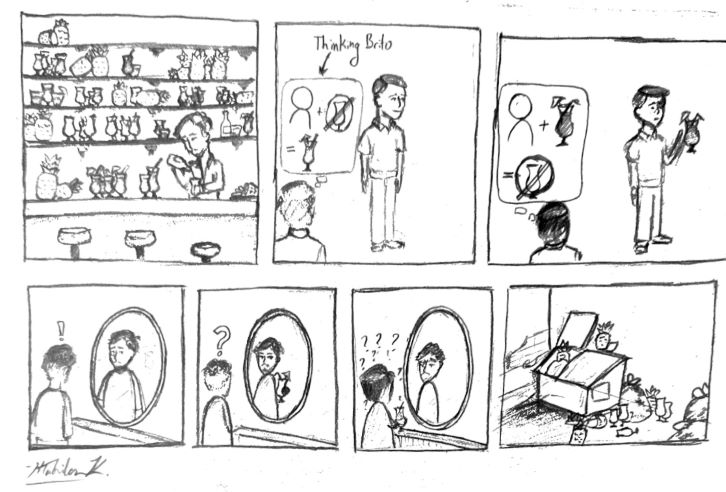
\includegraphics{PinaColada.jpg}}
\caption{Brito's Dilemma}
\label{Pina Colada Situation Image}
\end{figure}

\subsection{From Drinks to Mathematics}
Brito's dilemma, while amusing, hints at a much greater philosophical problem: the paradox of \emph{\textbf{self-reference}}. When logical systems create statements that refer to themselves, paradoxes often emerge. In the case of Brito's piña colada situation, self-reference was introduced when Brito used his own state to make decisions his own state. 

If we can formalize another logical system (mathematics, for example) in a way that allows for self-reference, we can create a similar paradox. Gödel achieves this by using Gödel numbers to represent mathematical statements. From there, he formally constructs the self-referential statement, "this statement cannot be proven," which is often labeled \textit{G}. 

If \textit{G} is false, then it can be proven that \textit{G} cannot be proven; this cannot be the case, because it yields a contradiction. That means that \textit{G} must be true, and there exist mathematical statements, namely \textit{G}, that cannot be proven (i.e. mathematics is incomplete). 

\section{Background}
Naturally, the previous few sections provide some nice intuition towards Gödel's Incompleteness Theorem but do not provide rigorous proof. We offer such proof in Section III, to formalize the notion of self-reference. However, before we can begin, we must cover some necessary background information on completeness and Gödel Numbering. 

\subsection{Completeness}
In order to understand Gödel's Incompleteness Theorem, one must first define what it means for a formal system to be complete (and what a formal system is, in the first place). 

A formal system is a system of axioms combined with rules of inference that enables the creation of new theorems. A \emph{\textbf{consistent}} system, the only kind of system relevant here (as inconsistent systems are trivially complete), is one in which a theorem and its negation can't both be proven (i.e. the Law of Non-Contradiction is maintained). A formal system is \emph{\textbf{complete}} if every statement or its negation but not both can be derived in the system. 

\subsection{Gödel Numbers}
In order to formalize self-referential statements in mathematics, we utilize Gödel Numbering. Let $k$ mathematical symbols each correlate to a natural number from 1 to $k$, and $x$ variables correlate each to a prime number greater than $k$ as such:
\begin{table}[htbp]
\caption{Symbol to Gödel Number Conversions}
\begin{center}
\begin{tabular}{ |c|c||c|c| } 
 \hline
 Symbol & Number & Symbol & Number \\ 
 \hline
 \hline
 '0' & 1 & '$\neg$' & 9 \\ 
 \hline
 '$'$' & 2* & '$\forall$' & 10 \\ 
 \hline 
 '+' & 3 & 'x' & 11 \\ 
 \hline
 'x' & 4 & 'y' & 13 \\ 
 \hline
 '=' & 5 & 'z' & 17 \\ 
 \hline
 '(' & 6 & 'a' & 19 \\ 
 \hline
 ')' & 7 & 'b' & 23 \\ 
 \hline
 '$\rightarrow$' & 8 & 'c' & 29 \\ 
 \hline
 
\end{tabular}
\end{center}
\begin{center}
    *Note: This symbol ($'$) denotes the successor function. This is the function that takes in a natural number and maps it to itself plus 1. For example, \[0' = 0 + 1 = 1\]
    
\end{center}
\end{table}

We seek to assign a unique numerical representation to each mathematical formula (aka. number them) so that we can analyze the properties of the set of all formulas.

We can assign each mathematical formula of length l a number by creating the prime factorization: 

\[2^{i_1}*3^{i_2}*5^{i_3}*...*p_l^{i_l}\] 

Where each i represents the number correlating to each symbol in the mathematical formula. For example, the formula $0=0$ can be represented with $2^1*3^5*5^1$ which is equivalent to the number 2340. Because of the Fundamental Theorem of Arithmetic, each formula will be given a different number as each will have a unique prime factorization. We will denote the Gödel Number of a Formula $A$ with $\lceil A \rceil$ or, alternatively, $a$. We've created an Java application for converting between Gödel numbers and statements; the code for this application can be found in the appendix. 

The next key ingredient to Gödel's proof is the meta-analysis of symbols made possible through Gödel numbering. For example, if we wish to discuss the set of formulas that begin with the $\neg$ symbol, we could build the set of relevant Gödel numbers with:

\[\{x \in \mathbb{N} \; : \;2^9\mid x \; \land \; 2^{10} \nmid x\}\]

This logic carries forward into functions that transform formulas into their negations ($f(
\lceil A \rceil ) = \lceil \neg A \rceil$), send two formulas A and B to their implication ($impl(\lceil A \rceil , \lceil B \rceil ) = \lceil A \rightarrow B \rceil$), and so forth for all syntactic operations and analyses. There are even functions that identify whether given formulas are truly given axioms and rules of inference. These functions can be chained and combined into a function that identifies whether a series of formulas exists such that a given formula can be proven. We will call this formula $Prov_F$.

\subsection{Introducing Self-Reference}
The final ingredient to Gödel's Theorem is self-reference. Let us exclusively analyze formulas with a single variable (WLOG, we will use $x$). Gödel numbering will allow us to identify a unique representation number for each formula, and each formula will contain at least one prime raised to 11, the Gödel number representing $x$:
\[2^{i_1}*3^{i_2}*5^{i_3}*...*p_x^{\textbf{11}}*...*p_l^{i_l}\]

For example, the formula $x=x'$ can be represented as $2^{\textbf{11}}*3^5*5^{\textbf{11}}*7^2 = 1.1907*10^{15}$. As we can substitute any number for $x$ and still have a valid formula, in any equation with $x$, we can substitute all powers representing $x$ (all powers of exactly 11) with a different number. To achieve self-reference, we simply substitute a formula's Gödel number into itself:
\[\{x=x'\} \rightarrow \{(1.1907*10^{15}) = (1.1907*10^{15})'\}\]
Note that the x's have been replaced by the relevant Gödel number. This operation under Gödel numbering (as opposed to the raw equation) is similar:
\[\{2^{\textbf{11}}*3^5*5^{\textbf{11}}*7^2\} \rightarrow \{2^{1.1907*10^{15}}*3^5*5^{1.907*10^{15}}*7^2\}\]
Note that the bolded 11's from the previous equation have been replaced with the relevant Gödel number. More Generally, this follows the form:
\[\{\lceil B(x)\rceil\} \rightarrow \{\lceil B(\lceil B\rceil )\rceil\}\]

While in the above operation, this self-reference is arbitrary, as the equation $x=x'$ has no concept of the meaning of Gödel Numbering, this substitution becomes critically important when the formula being altered can make reference to the rules of Gödel Numbering. 

\section{Proof}
The proof of the Incompleteness theorem uses a self-referencing Gödel function which, in Layman's terms, translates to "this statement is not provable" to demonstrate that mathematics is incomplete. We will begin with the construction of an engine for self-reference which translates to "this statement is $A$" where $A(x)$ is an arbitrary function. We will then use the $Prov_F$ function to create a paradoxical statement which demonstrates the incompleteness of a simple mathematical system $F$.

Let $S(x, y)$ be the function that determines whether $y$ is the Gödel Number created by substituting $x$ into itself. The following table demonstrates some example inputs using arbitrary functions $H(x)$ and $T(x)$. The first two input rows are identical with different notation.
\begin{center}
\begin{tabular}{ |c|c||c| } 
 \hline
 $x$ & $y$ & $S(x,y)$\\ 
 \hline
 \hline
 $h$ & $\lceil H(h) \rceil$ & true \\ 
 \hline
 $\lceil H(x)\rceil$ & $\lceil H(\lceil H(x) \rceil)\rceil$ & true\\ 
 \hline 
 $h$ & 123 & false \\ 
 \hline
 123 & $\lceil H(h) \rceil$ & false \\ 
 \hline
 $h$ & $\lceil T(h)\rceil$ & false \\ 
 \hline
 
\end{tabular}
\end{center}

Using the aforementioned arbitrary formula $A(x)$, $B(x)$ is defined:
\[B(x) = \exists y(A(y) \land S(x,y))\]

Note that this essentially translates, given the rules of Gödel numbering, to there is a y which is the number of a self-referencing Gödel formula (ie. $y = \lceil H(\lceil H(x) \rceil) \rceil$) and $A(y)$ is true. We will now substitute $\lceil B(x) \rceil$ (Represented here as $b$) for $x$ to yield:

\[B(b) = \exists y(A(y) \land S(b,y))\]

Because Gödel numbers are unique, we can identify that the only valid $y$ for this equation is $\lceil B(b) \rceil$. This is demonstrable because any other value of $y$ would lead S(b, y) to be false -- as S(x, y) determines whether $y$ is the self-reference construction of $x$. For sake of simplicity, we will denote the self-referential $B(b)$ as $D$, such that $y = \lceil D \rceil$. This alteration yields:
\[D = \exists y(A(y)\land S(b,y))\]

Let us assume that a system of mathematics we are interested in, $F$, is complex enough to contain the above reasoning. Because $F$ can demonstrate that the only possible $y$ is $d$, we can rearrange the equation to remove the quantifier and replace $y$ with $d$.
\[D = A(d) \land S(b, d)\]

Because of $b$ and $d$ form the correct self-referential relationship by design, $S(b, d)$ is true and can be removed via the identity law:
\[D = A(d)\]

Because these reductions were made under the laws of $F$, we recognize that $F$ proves the above statement, or, in logical notation:
\[F \vdash D \leftrightarrow A(d)\]
Note that $\vdash$ represents "proves", and $\leftrightarrow$ replaces the equals sign from the prior equation. 

Since $A$ is an arbitrary function, we can substitute any function in for $A$ and this relationship will still be true. This is the engine from which Gödel discusses a statement within itself. For example, if $A$ was the function which determines whether the inputted Gödel number begins with a $\neg$ symbol, this would translate to ($F$ proves) "$D$ iff $D$ begins with $\neg$". In other words, ($F$ proves) "this statement begins with $\neg$". Note that both versions of this statement are logically equivalent.

Recall the formula from earlier which determines whether a given statement is provable under $F$, $Prov_F$. We can substitute the negation of this formula: $\neg Prov_F$ for $A$. We will call this new statement $G$:
\[F \vdash G \leftrightarrow \neg Prov_F(g)\]

In layman's terms, this translates to: $F$ proves that "this statement is not provable under $F$" where $G$ is the statement in quotes. From this point, it is easy to identify the contradiction through which Gödel identifies Incompleteness. If $G$ is true than it is not provable under $F$. If $G$ is false, then it is provable and, thus, true. This is a contradiction; therefore, we resort to the former conclusion and $F$ is incomplete.

An observant reader may notice at this point that a second contradiction can be identified: If $G$ is proved to be true, then that very proof contradicts with $G$'s assertion that it is not provable. The barrier preventing this contradiction is the scope of $F$. $F$ is not a complex enough system to contain Gödel's proof, thus preserving its consistency. If it were, the system would be provably inconsistent, a problem elaborated on in Section IV.B: Gödel's Second Proof.

\section{Discussion}
\subsection{Implications for Mathematics}
On a broad scale, Gödel’s results have tremendous ramifications for mathematics as a whole. Over the course of this class, we’ve discussed, referenced, or touched upon dozens of open problems. The Twin Prime Conjecture, the Riemann Hypothesis, the Collatz Conjecture, and NP=P are just a few of the thousands of currently-unproven mathematical theorems. Solving just one of these (consider NP=P, for example) would have a drastic effect on mathematics and the sciences as a whole, likely leading to a surge in technological progress and development. 

Yet, Gödel’s special statement indicates that any consistent system of mathematics contains true statements that cannot be proven! As such, not only might we be currently lacking the appropriate mathematical intuition or lemmas to prove any of the above statements; it might be physically impossible to prove those statements under any system of mathematical reasoning at all.

No matter how many careers are spent analyzing the Twin Prime Conjecture or the Riemann Hypothesis, we may never be able to confidently convince ourselves that these statements are true. We may never be able to use them to logically intuit other facts about mathematics. We may never be able to build off of them to generate new knowledge. We may never be able to utilize them to model the natural world. Our system of mathematics—any system of mathematics—cannot be complete. 

\subsection{Gödel's Second Proof}
After publishing his first proof of incompleteness, Gödel went on to use his established numbering system to analyze the consistency of mathematical systems. Recall that a consistent system is one where a theorem and it's negation can't both be proven. The opposite, an inconsistent system, must have some statement $p$ where both $p$ and $\neg p$ can be proven (i.e. inconsistent systems yield logical contradictions and are thus incorrect). 

In his second proof, Gödel demonstrates that any consistent mathematical system can only prove its own consistency if it is, in fact, inconsistent. Essentially, we can only prove that our system of mathematics is free of logical errors if our system of mathematics has logical errors. Ironically, one of those logical errors would be the proof of consistency itself.

Let's briefly discuss how Gödel arrived at this result. Based on the First Incompleteness Theorem, we know that there exists a statement $G$ that is equivalent to "this statement cannot be proven." If we're able to prove $G$, then our system of mathematics is inconsistent (for the same reasons explored in Gödel's First Incompleteness Theorem). 

Thus, to have a consistent mathematical system, $G$ cannot be proven. So to prove that our system of mathematics is consistent, we must prove that $G$ cannot be proven. But the statement "$G$ cannot be proven" is, in fact, $G$. And the only way to prove $G$ is with an inconsistent system of mathematics.

We've reached a contradiction. A system of mathematics can only prove its own consistency if it's already inconsistent. Thus, Gödel's Second Incompleteness Theorem marked the end of the search for a mathematical system that was both complete and consistent. 

\subsection{Hilbert's Program for Mathematics} 
During the early 1900s, many mathematicians were re-examining earlier mathematical proofs and were horrified to find multiple logical errors in their reasoning. To solve this problem, David Hilbert (who discovered a space-filling curve, among other profound results) laid out his vision for a formal, unambiguous method of proofs called Hilbert's Program. This system lays out the rules, axioms, and propositional logic that we use for mathematical proofs to this day. Hilbert hoped that this new formal, unambiguous system of mathematics would satisfy three basic properties: 

\begin{enumerate}[]
    \item \emph{Completeness}
    \item \emph{Consistency}
    \item \emph{Decidability}
\end{enumerate}

Gödel's first incompleteness theorem disproved the "completeness" quality, demonstrating that a consistent mathematical system cannot be a complete one. Gödel's second incompleteness theorem demonstrated that it is impossible for any consistent system of mathematics to prove its own consistency. \emph{\textbf{Decidability}}, which we have not yet discussed, is the idea that there exists an algorithm that can decide the truth or falsehood of every mathematical statement. Turing's work on the halting problem later put the decidability of our mathematical systems into question.

\subsection{The Halting Problem}
During and after the publications of Gödel's theorems, Alan Turing was studying a similar problem in computer science. Turing envisioned a machine that could read, write, and move between inputs from an infinitely long set of 1s and 0s using instructions from a state-based program; the device he imagined can actually do everything that a modern computer can, a property called \emph{\textbf{Turing-completeness}}, but proving that is perhaps beyond the scope of this project.

Programs fed to this machine could either run infinitely or stop after some finite number of instructions. Turing was trying to determine if it was possible to create a program that could determine whether any other program would halt or run infinitely given a particular input. Using a similar self-referencing tactic to Gödel's, Turing was eventually able to create a contradiction using the following program outlined in Algorithm 1, thus proving that no such $halts()$ program can exist: 

\begin{algorithm}[H]
\begin{algorithmic}
\caption{Turing's Contradictory Program}\label{alg:cap}
\If{halts(self)}
    \State{$loop\_infinitely()$}
\Else
    \State{$halt$}
\EndIf
\end{algorithmic}
\end{algorithm}

Beyond their strategic similarity, Gödel's Incompleteness Theorem and Turing's solution to the Halting Problem are fundamentally intertwined. One may consider Turing's results as a reformulation of Gödel's work in terms of algorithms. Conversely, one may consider that Gödel's Incompleteness Theorem looks at mathematics as a Turing-complete system to create an analog to the halting problem. Indeed, one may construct a proof for a slightly weaker version of Gödel's Incompleteness Theorem based on the results of the Halting Problem. This allows us to generalize (with some restrictions) the basic intuition behind Gödel's results to any Turing-complete system.  

\subsection{Quantum Systems (and Magic the Gathering)} 
More recently, a team of several quantum physicists [11] were analyzing the spectral gap (the gap between the lowest-energy and next-lowest-energy states of a material). Depending on the structure and chemical properties of a given material, the lower-energy states may be continuous and this gap may not even exist. The physicists described above were trying to design an algorithm to determine whether the gap existed for a particular material based on its structure.

To start, the physicists analyzed a hypothetical, arbitrary 2D crystal lattice of atoms. Through a 146 pages of mathematics, the physicists were able to prove that the spectral gap of this arbitrary material actually formed a Turing-complete system. In this case, their algorithm to determine whether the spectral gap existed was analogous to Turing's halting program (and was thus undecidable). Ultimately, these results imply that the algorithm the physicists set out to find does not exist. 

The results of this study are fascinating and generalize Gödel's and Turing's results to real-world physical systems. Interestingly, many other physical systems are similarly Turing-complete and undecidable (including \emph{Magic: The Gathering}).

\section*{Appendix}
In working on this project, we've created a Java application to convert between Gödel numbers and statements. Below, we've included the code used to run this application. 
\begin{lstlisting}[language=Java]
import java.math.BigInteger;
import java.security.PublicKey;
import java.util.HashMap;
import java.util.Map;
import java.util.Scanner;

public class Converter {
    static Map<Character, Integer> map = new HashMap<>();
    //initialize an array of primes with the first 200 hundred primes 
    public static int[] primes = new int[]{2, 3, 5, 7, 11, ... 1223};
    // 0 , ' , +, *, =, (, ), #, ~, @, xi

    public static void main(String[] args) {
        Scanner scan = new Scanner(System.in);
        //initialize a map between characters and their Godel numbers
        map.put('0', 1);
        map.put('\'',2);
        map.put('+', 3);
        map.put('*',4);
        map.put('=', 5);
        map.put('(',6);
        map.put(')',7);
        map.put('#', 8);
        map.put('~',9);
        map.put('@',10);
        map.put('x', 11);

        //prompt response
        /*
        
        Hello!
        Welcome to the Godel Number Converter
        Write a mathematical expression using
        the valid symbols:
        0 , ' , +, *, =, (, ), #, ~, @, xi
        note that # is the implication symbol
        and xi here is x sub which denotes the
        i-th variable.
        (NOTE: raw numbers inputted are not
        converted to the standard godel number
        of |0''...'| notation.)
        keep inputs less than 200 characters
        
        */
        System.out.println("Hello!\n" + ... );
        System.out.print("input: ");
        char[] input = scan.nextLine().replaceAll("\\s", "").toCharArray();
        long[] res = new long[input.length];
        int j = 0;
        //loops through each character and converts it to its Godel number according to the table
        for (int i = 0; i < input.length; i++) {
            long num;
            //if a variable is inputted this calculates the subscript of the variable 
            if (input[j] == 'x') {
                num = 11;
                long sub = 0;
                while (Character.isDigit(input[j])) {
                    sub = (sub * 10) + input[j];
                    j++;
                }
                num += sub;
            } else {
                num = map.get(input[j]);
            }
            res[i] = num;
            j++;
        }
        // prints out the list of exponents to be mapped to prime numbers
        printArr(res);
        System.out.println();
        System.out.println("godel number: " + calcGodel(res));
    }
    public static void printArr(long[] arr) {
        System.out.print("[");
        for (int i = 0; i < arr.length; i++) {
            System.out.print(arr[i]);
            if (i < arr.length - 1) {
                System.out.print(", ");
            }
        }
        System.out.print("]");
    }

    public static BigInteger calcGodel(long[] arr) {
        BigInteger res = new BigInteger("1");
        for (int i = 0; i < arr.length; i++) {
            res = res.multiply(new BigInteger(String.valueOf(primes[i])).pow((int) arr[i]));
        }
        return res;
    }
}
\end{lstlisting}
    
\begin{thebibliography}{00}
    \bibitem{b1} N. Wolchover, “How gödel's proof works,” Quanta Magazine, 14-Jul-2020. [Online]. Available: https://www.quantamagazine.org/how-godels-incompleteness-theorems-work-20200714/.
    \bibitem{b2} P. Raatikainen, “Gödel's incompleteness theorems,” Stanford \break Encyclopedia of Philosophy, 02-Apr-2020. [Online]. Available: https://plato.stanford.edu/entries/goedel-incompleteness/. 
    \bibitem{b3} "Math's Fundamental Flaw," YouTube. 22-May-2021. Avaliable: https://www.youtube.com/watch?v=HeQX2HjkcNo
    \bibitem{b4} M. Henriksen, “What is Godel's theorem?,” Scientific American, \break 25-Jan-1999. [Online]. Available:  https://www.scientificamerican.com/\break article/what-is-godels-theorem/. 
    \bibitem{b5} S. Flender, “The limits of knowledge,” Towards Data Science, 21-May-2020. [Online]. Available: https://towardsdatascience.com/the-limits-of-knowledge-b59be67fd50a. 
    \bibitem{b6} R. Zach, “Hilbert's program,” Stanford Encyclopedia of Philosophy, 24-May-2019. [Online]. Available: https://plato.stanford.edu/entries/hilbert-program/. 
    \bibitem{b7} “Gödel's second incompleteness theorem,” Wolfram MathWorld. \break [Online]. Available: https://mathworld.wolfram.com/GoedelsSecond\break IncompletenessTheorem.html. 
    \bibitem{b8} "Gödel's Incompleteness Theorem - Numberphile," YouTube. 31-May-2017. Avaliable: https://www.youtube.com/watch?v=O4ndIDcDSGc
    \bibitem{b9} "Gödel's Incompleteness Theorem (extra footage 1) - Numberphile," \break YouTube. 03-Jun-2017. Avaliable: https://www.youtube.com/watch?v=\break mccoBBf0VDM
    \bibitem{b10} "Gödel's Incompleteness Theorem (extra footage 2) - Numberphile," \break YouTube. 03-Jun-2017. Avaliable: https://www.youtube.com/watch?v=\break 7DtzChPqUAw
    \bibitem{b11} T. S. Cubitt, D. Perez-Garcia, and M. M. Wolf, “Undecidability of the Spectral Gap,” arxiv, Jul. 2018. 
\end{thebibliography}
\end{document}